\subsection*{Porcentaje de contribución}

Se definió una función $\gamma$ para medir el porcentaje de las dos componentes más grandes del gradiente en cada iteración de la optimización. La función $\gamma$ tiene la siguiente forma

\begin{equation*}
    \gamma(g_k) = \frac{|g_k^{(1)}|+|g_k^{(2)}|}{\sum\limits_i |g_k^{(i)}|}
\end{equation*}

Realizando el calculo de la función $\gamma$ con la función lambda en el punto inicial $x=(10,10,\dots,10)^T$ se obtuvieron los resultados mostrados en la figura \ref{fig:gamma} para los diferentes métodos.

\begin{figure}[H]
    \begin{subfigure}{8.4cm}
        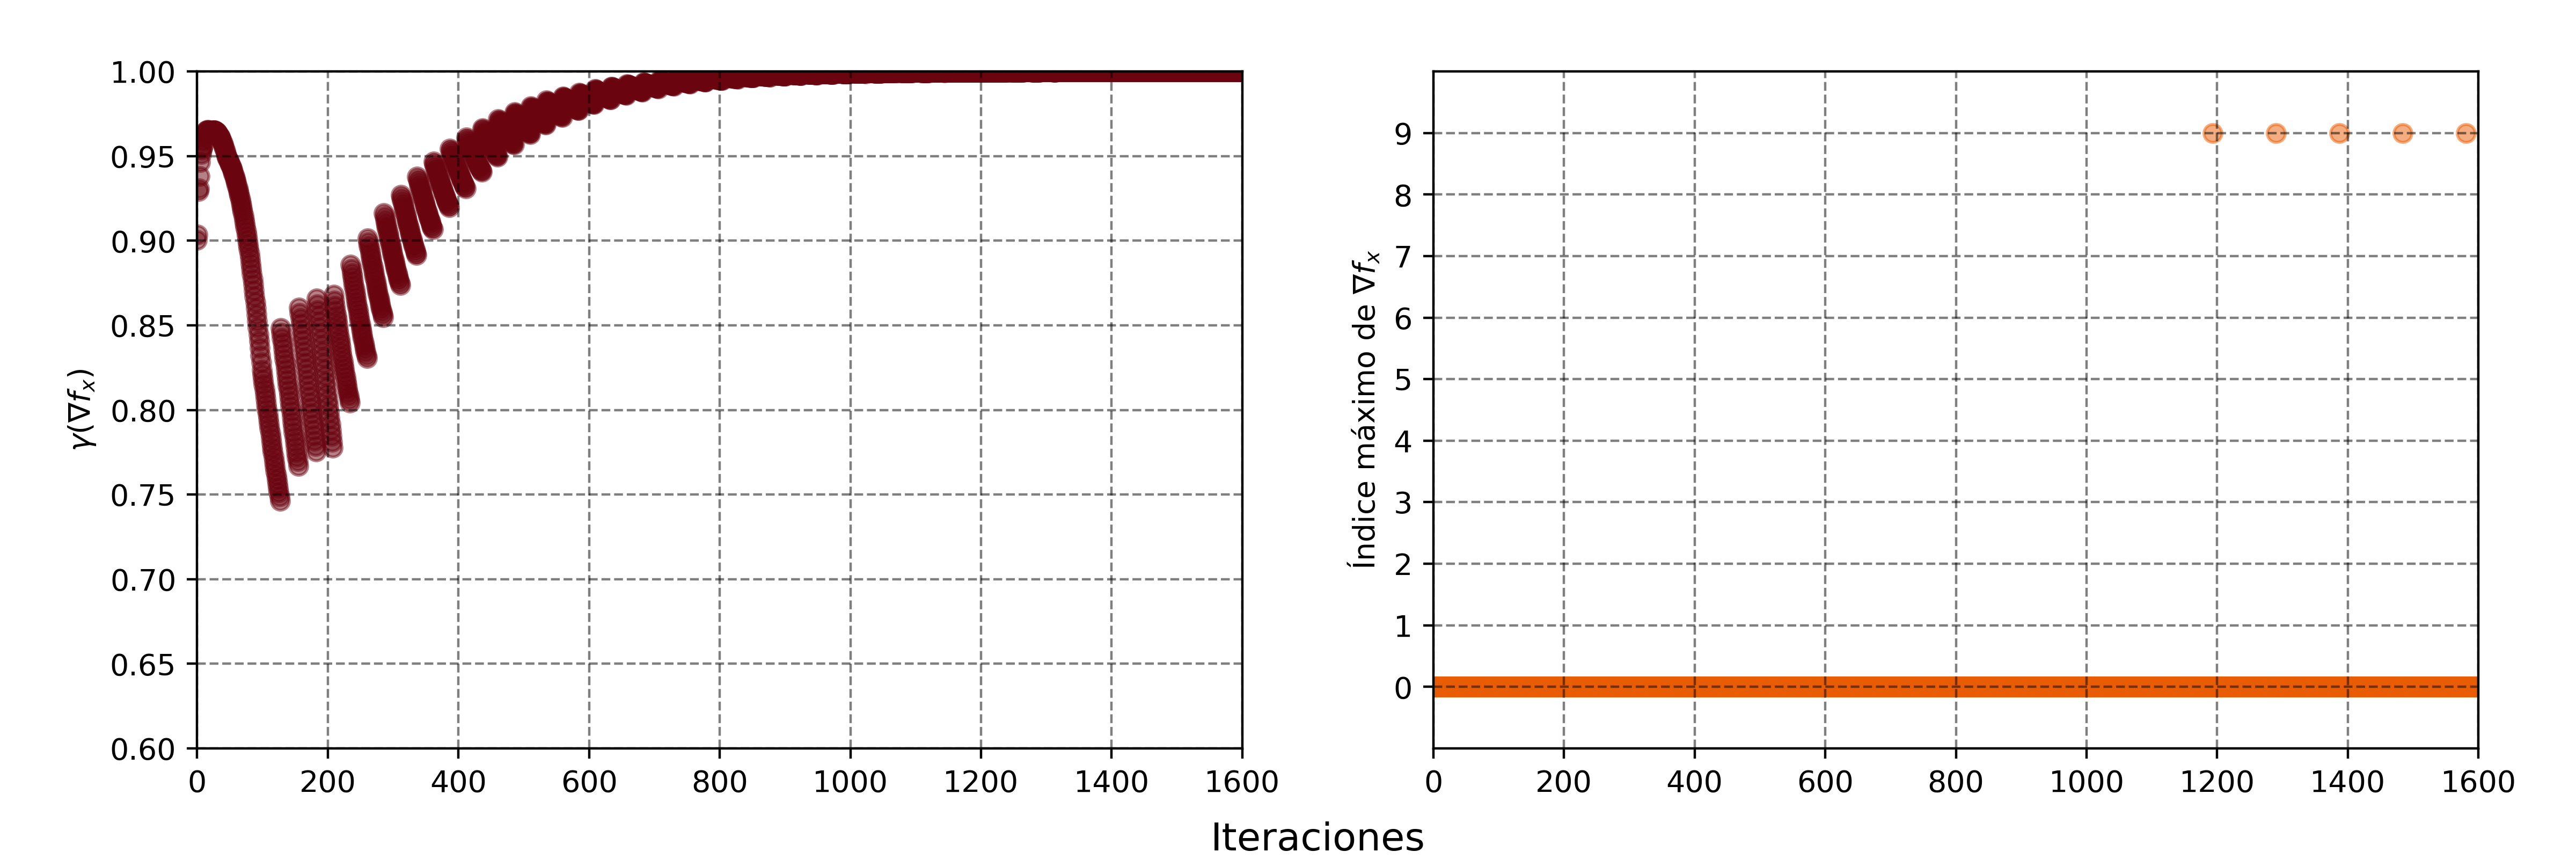
\includegraphics[width=1\textwidth]{graphics/gamma/steepest.png}
        \caption{Método de descenso de gradiente.}
    \end{subfigure}
    \begin{subfigure}{8.4cm}
        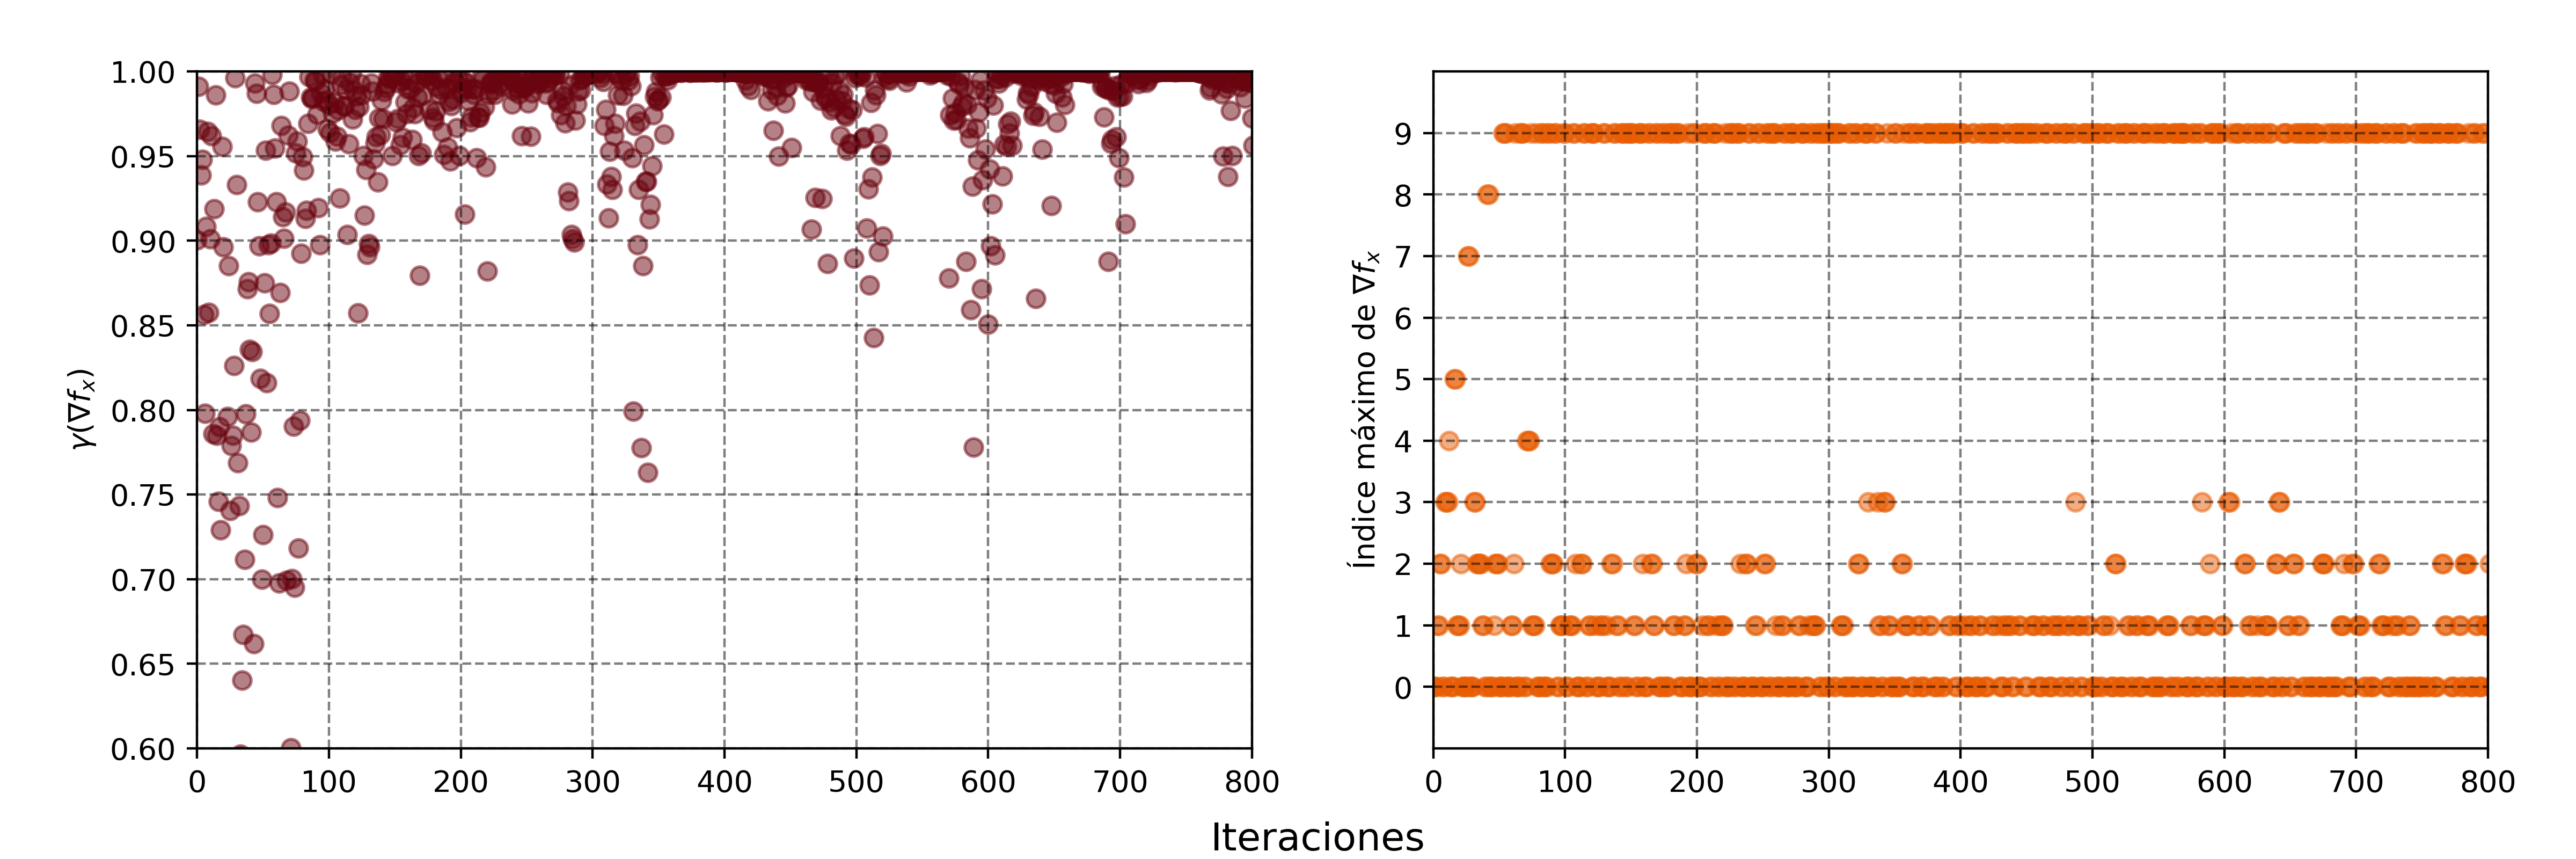
\includegraphics[width=1\textwidth]{graphics/gamma/barzilai.png}
        \caption{Método BB.}
    \end{subfigure}
    \begin{subfigure}{8.4cm}
        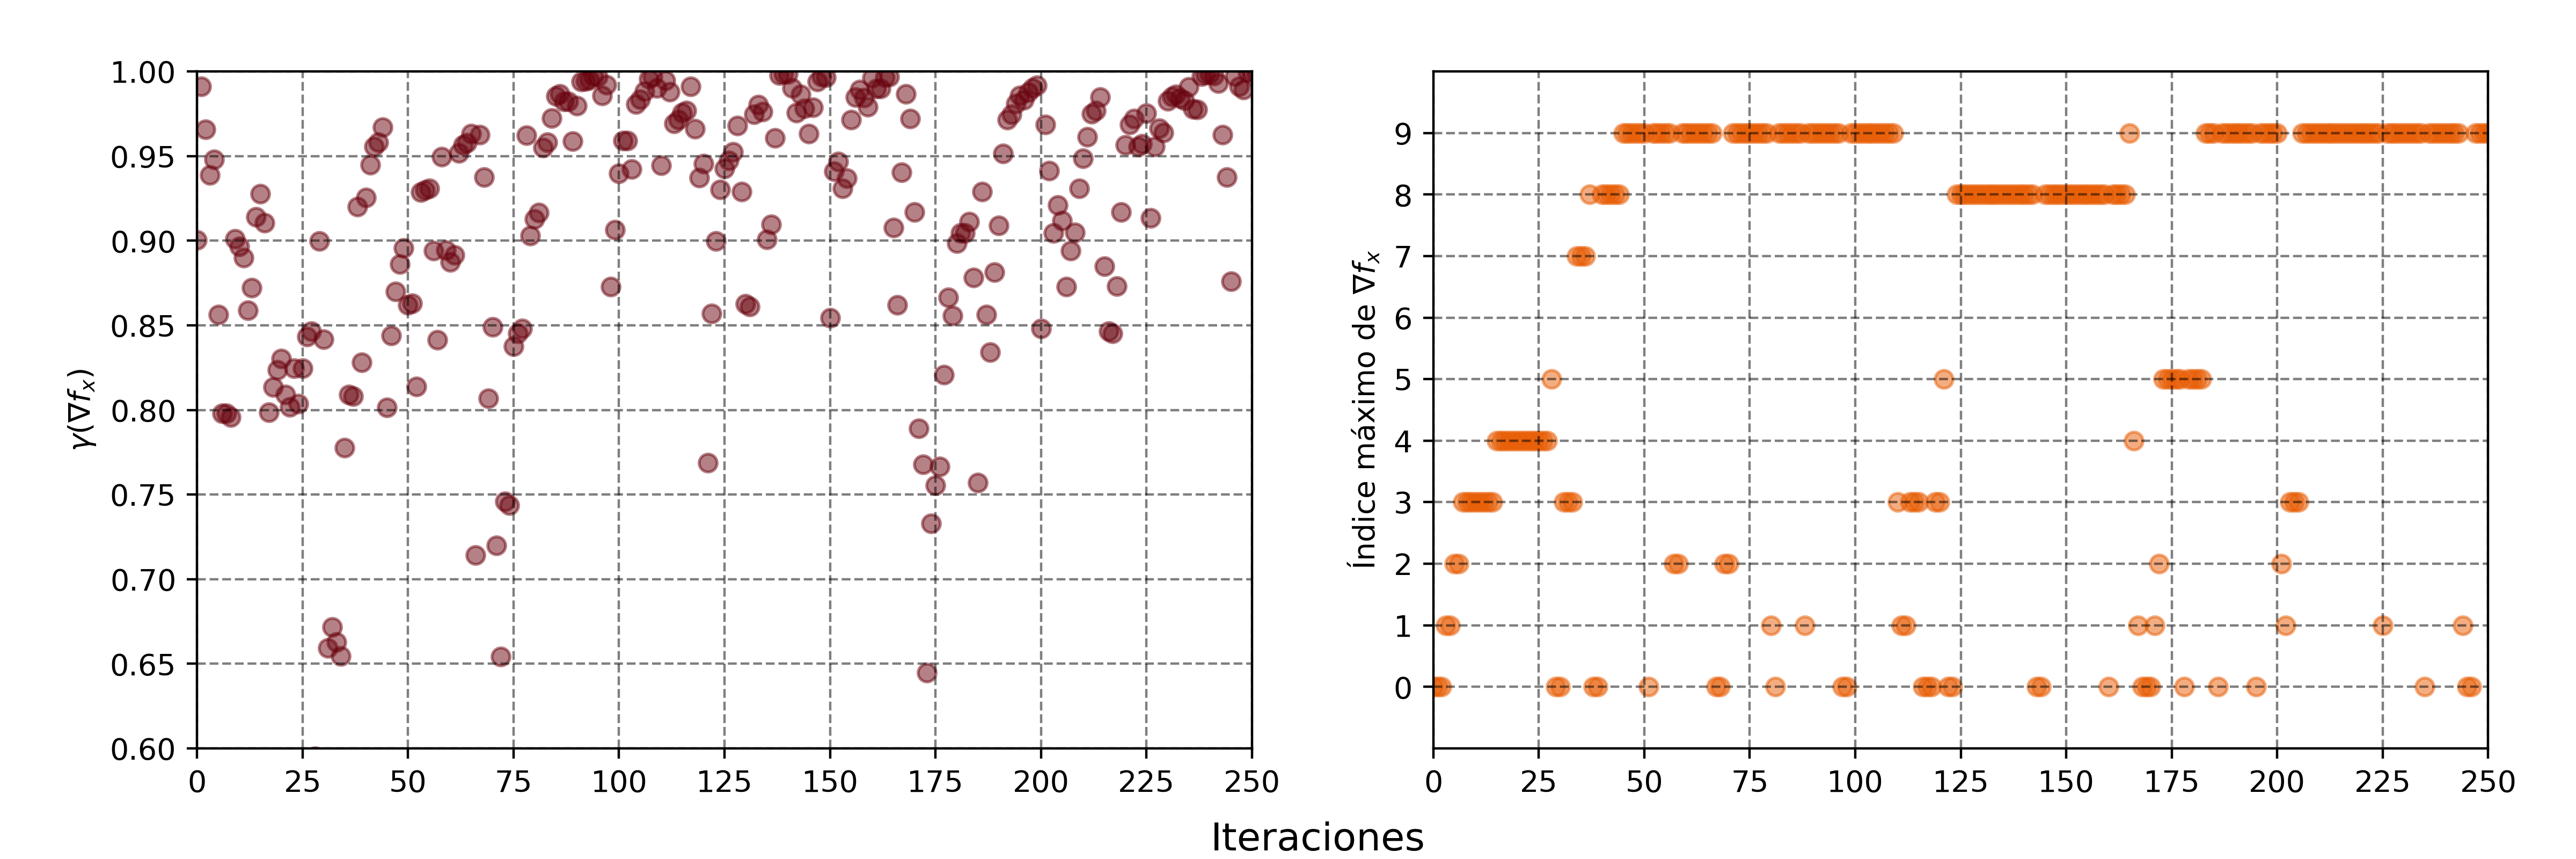
\includegraphics[width=1\textwidth]{graphics/gamma/ANGM.png}
        \caption{Método ANGM.}
    \end{subfigure}
    \begin{subfigure}{8.4cm}
        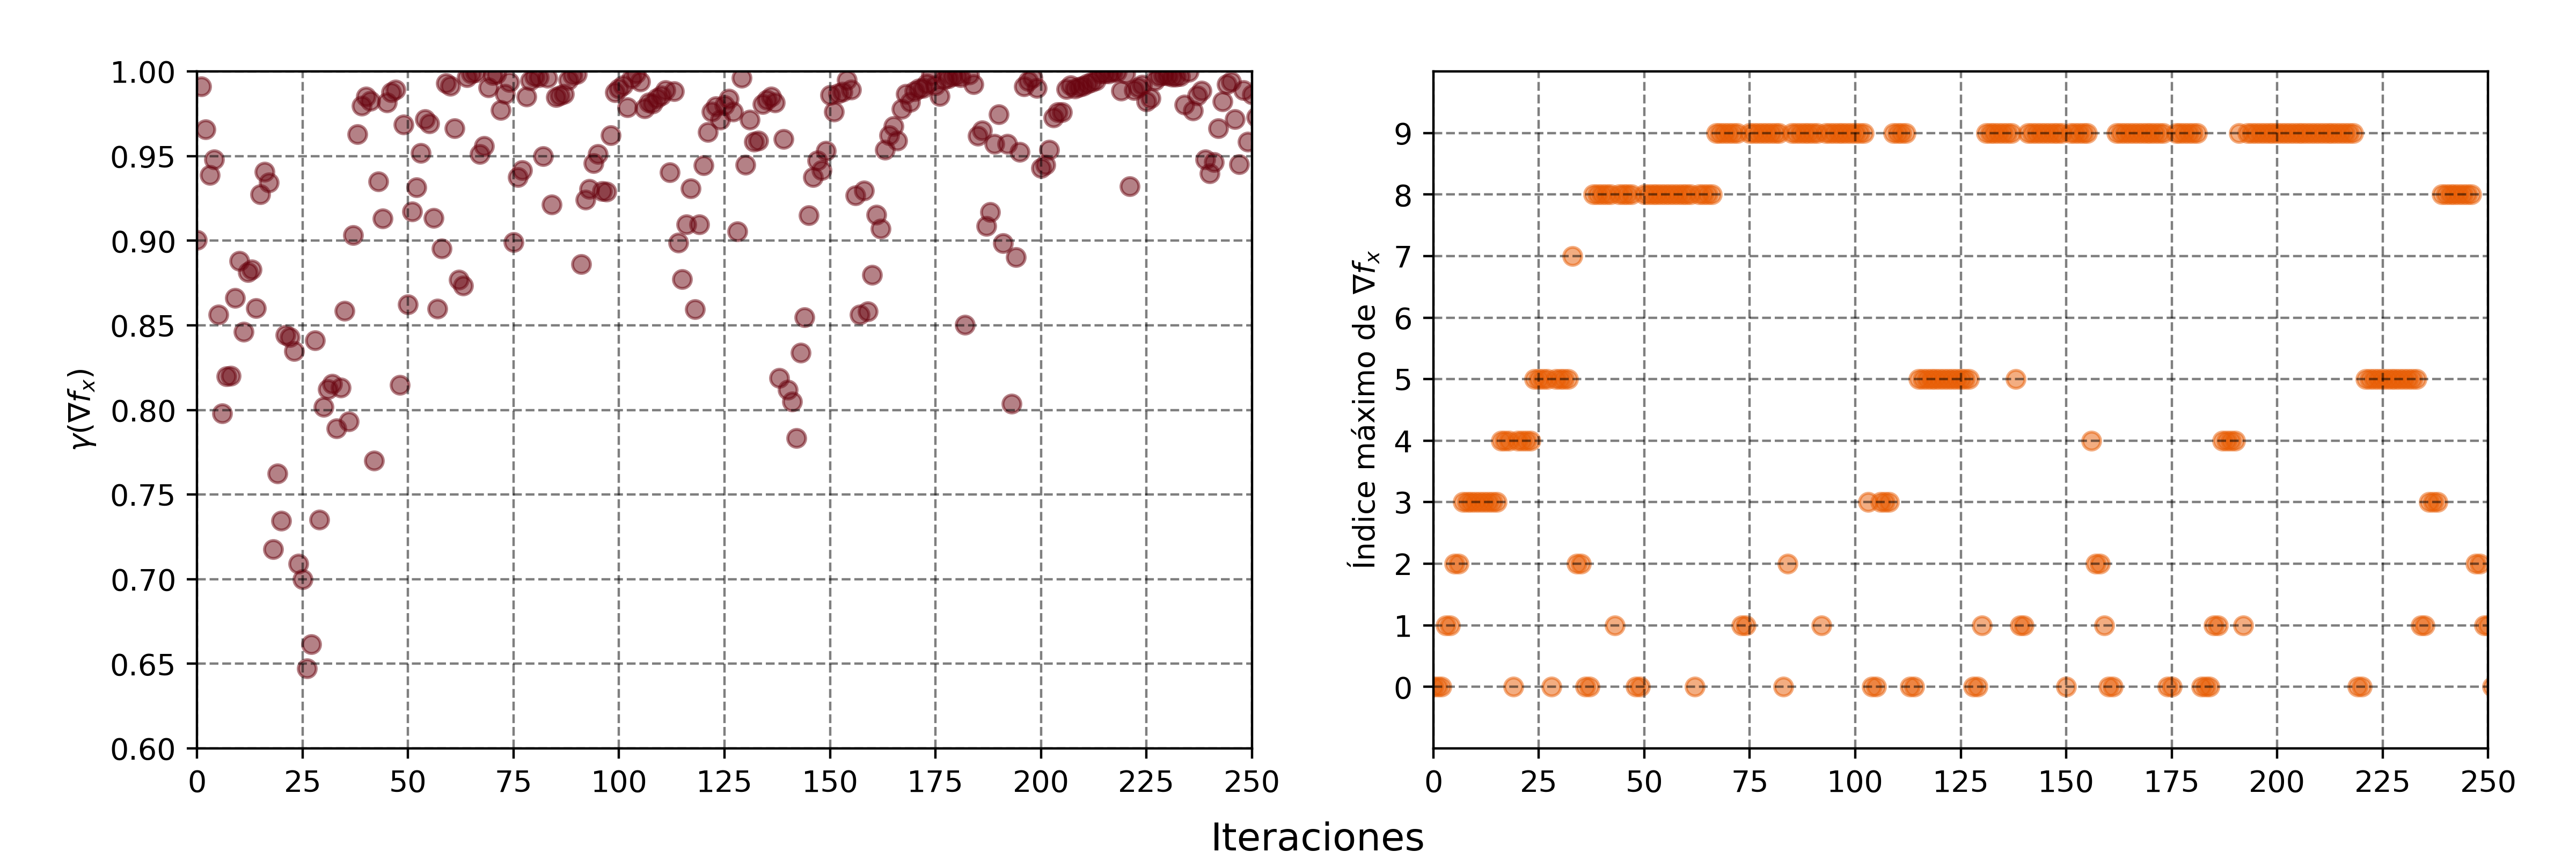
\includegraphics[width=1\textwidth]{graphics/gamma/ANGR1.png}
        \caption{Método ANGR1}
    \end{subfigure}
    \begin{subfigure}{16.5cm}
        \centering
        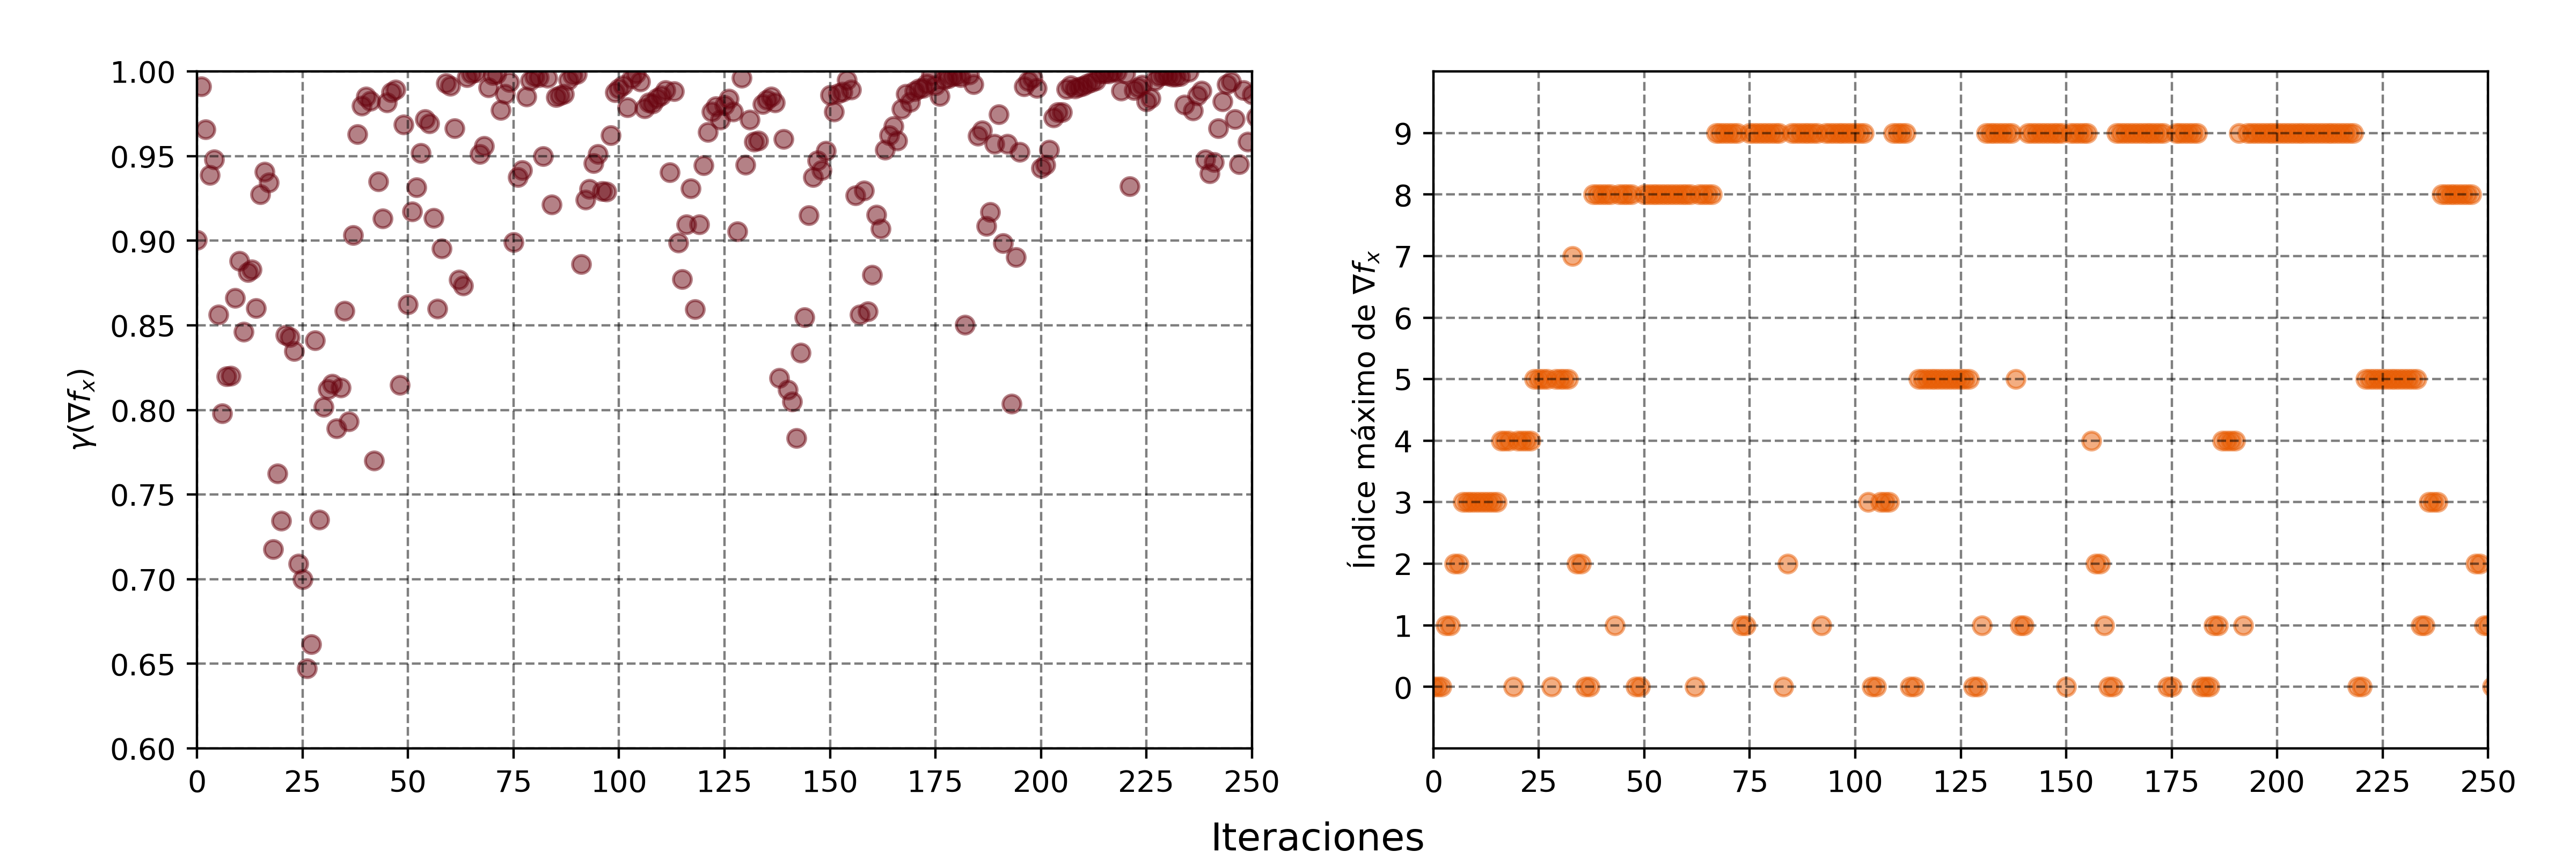
\includegraphics[width=8.4cm]{graphics/gamma/ANGR1.png}
        \caption{Método ANGR2.}
    \end{subfigure}
    \caption{Función $\gamma$ para diferentes métodos (izquierda) y la posición en el vector de la componente más grande (derecha).}
    \label{fig:gamma}
\end{figure}

En la tabla \ref{table:gamma_function} se muestra el número de iteraciones en las que se obtuvo un valor mayor a 0.8 para la función $\gamma$ en cada métodode optimización.

\begin{table}[H]
    \centering
    \begin{tabular}{lrr}
        \hline
        \textbf{Método} & $\boldsymbol{\gamma(g_k)>0.8}$ & \textbf{Total} \\\hline
        SD              & 8057                           & 8104           \\
        BB              & 815                            & 851            \\
        ANGM            & 293                            & 316            \\
        ANGR1           & 240                            & 253            \\
        ANGR2           & 200                            & 245            \\ \hline
    \end{tabular}
    \caption{Número de iteraciones donde el valor de la función $\gamma$ tuvó un valor mayor a 0.8 para cada método de optimización.}
    \label{table:gamma_function}
\end{table}